
Since previous work showed a degree of dependence on different ASV systems, seven different ... 

We assessed the impact of each spoofing attacks on seven popular ASV systems: (i) a standard GMM-UBM system with 1024 Gaussian components, as the one used e.g., in~\cite{Roy2012} (ii) a GMM supervector linear kernel (GSL) system, (iii) a GSL system with nuissance atribute projection (NAP) used for channel compensation~\cite{Campbell2006}, (iv) a GSL with factor analysis (FA) ~\cite{Fauve2007}, (v) a GMM-UBM system with factor analysis, (vi) an iVector system~\cite{Dehak2011}, and (vii) an iVector system  with probabilistic linear discriminant analysis (PLDA)~\cite{Li2012} and length normalisation~\cite{Garcia2011}. A comprehensive comparison of various channel compensation techniques used with GSL kernels can be found, e.g., in~\cite{McLaren2010}.

From here on in, the pure iVector system is referred to as IV system, whilst the state-of-the-art iVector system with PLDA is referred to as the IV-PLDA system. All seven ASV systems were tested with and without normalisation. The IV and IV-PLDA systems used symmetric score normalisation (S-norm) as described in~\cite{Kenny2010}, while the remaining systems utilised standard T-norm normalisation~\cite{Auckenthaler2000}.

All ASV systems used a common speech activity detector which fits a 3-component GMM to the log-energy distribution and which adjusts the speech/non-speech threshold according to the GMM parameters~\cite{Bimbot2004}.  Such an approach has been used successfully in many independent studies~\cite{magrin2001,fauve2008} and performed well in comparison to alternatives~\cite{sahidullah2012}. 

All ASV systems were based on the LIA-SpkDet toolkit~\cite{Bonastre2008} and the ALIZE library~\cite{Bonastre2004} and were directly derived from the work in~\cite{Fauve2007}.  They furthermore used a common UBM with 1024 Gaussian components and a common feature parametrisation: linear frequency cepstral coefficients (LFCCs), their first derivatives and delta energy.  

%% not sure if we can leave the below line as it reveals the authorship...
%Full details of the setup can be traced through~\cite{alegreBTAS2013}.



\begin{figure}
	\centering
	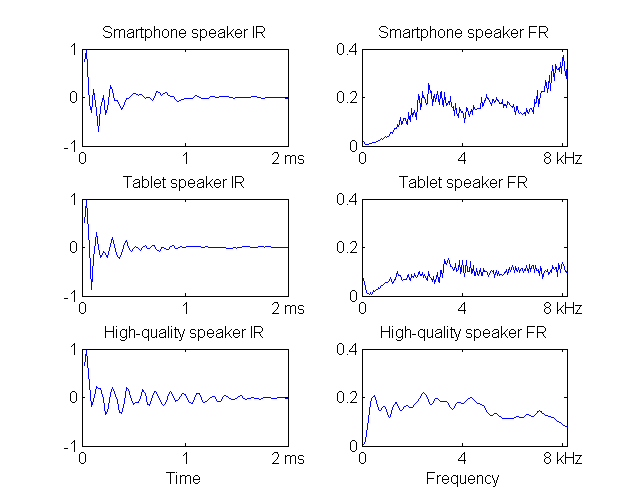
\includegraphics[width=1\linewidth]{Figs/IRs.png}
	\caption{Impulse responses (left) and corresponding frequency transmittance (right) of the three speakers used for playback emulation.}
	\label{fig::IRs}
\end{figure}


\begin{figure}
	\centering
	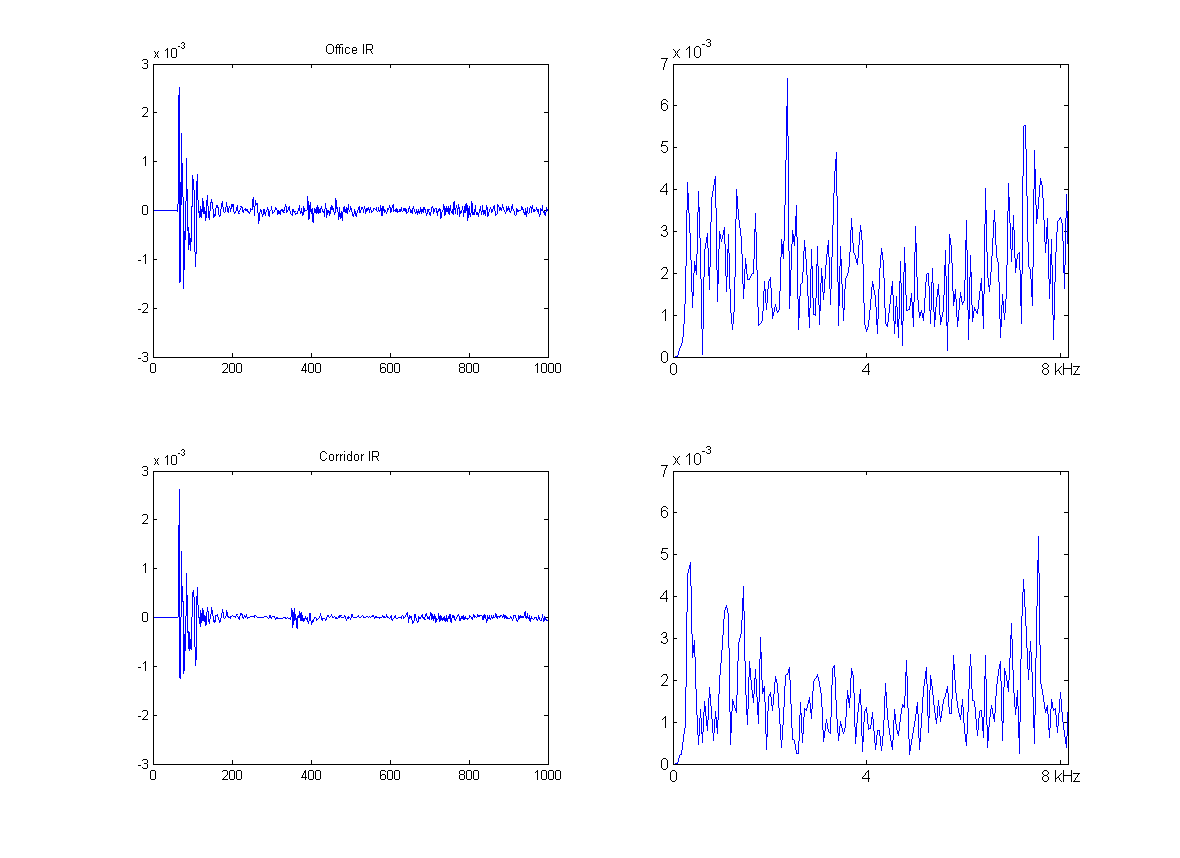
\includegraphics[width=1\linewidth]{Figs/Room_IRs.png}
	\caption{Impulse responses (left) and corresponding frequency transmittance (right) of the office and the corridor used for playback emulation.}
	\label{fig::Room_IRs}
\end{figure}



